\chapter{刚体力学}
\section{作业习题}
\subsection*{一、填空题}
\begin{enumerate}
    \item 如图 \ref{fig:34}, 一长为$L$, 质量为$m$的匀质细杆, 两端分别固定质量为$m$和$2m$的小球,
    此系统在竖直平面内可绕过中点$O$且与杆垂直的水平光滑固定轴($O$轴)转动. 
    开始时杆与水平成$60^\circ$角, 处于静止状态 . 
    无初转速地释放以后, 杆球这一刚体系统绕$O$轴转动. 
    释放后, 当杆转到水平位置时, 刚体受到的合外力矩$M=\nl$.
    \begin{figure}[H]
        \centering
        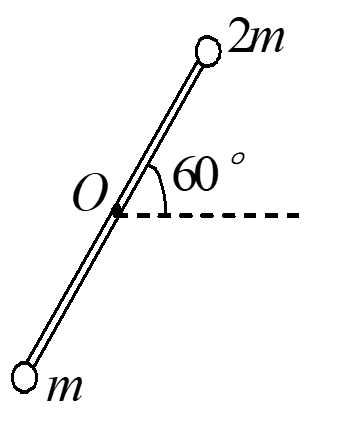
\includegraphics[width=0.15\textheight]{fig34}
            \caption{如图}\label{fig:34}
    \end{figure}
    \item 如图 \ref{fig:35}, 一定滑轮质量为$M$、半径为$R$, 对水平轴的转动惯量$J=(1/2)MR^2$.
    在滑轮的边缘绕一细绳, 绳的下端挂一物体. 
    绳的质量可以忽略且不能伸长, 滑轮与轴承间无摩擦, 
    物体下落的加速度为$a$.则绳中的张力$T=\nl$.
    \begin{figure}[H]
        \centering
        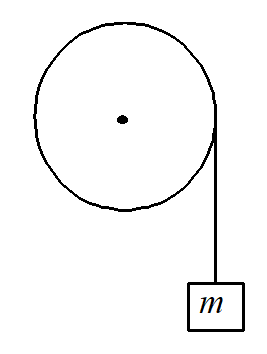
\includegraphics[width=0.15\textheight]{fig35}
            \caption{如图}\label{fig:35}
    \end{figure}
    \item 一长为$L$质量为$m$的均质细杆, 两端附着质量分别为$m_1$和$m_2$
    的小球, 且$m_1>m_2$, 两小球直径$d_1$、$d_2$都远小于$L$, 
    此杆可绕通过中心并垂直于细杆的轴在竖直平面内转动, 
    则它对该轴的转动惯量为\nl, 若将它由水平位置自静止释放, 
    则它在开始时刻的角加速度为多大\nl.

    \item 如图所示 \ref{fig:36}, 一质量为$m$的质点自由落下的过程中某时刻具有速度$V$,
    此时它相对于$A$、$B$、$C$三个参考点的距离分别为$d_1、d_2、d_3$
    则质点对这三个参考点的角动量的大小, $L_A=\nl$, 
    $L_B=\nl$, $L_C=\nl$; 作用在质点上的重力对这三个点的力矩大小,
    $M_A=\nl$; $M_B=\nl$; $M_C=\nl$.
    \begin{figure}[H]
        \centering
        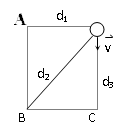
\includegraphics[width=0.15\textheight]{fig36}
            \caption{如图}\label{fig:36}
    \end{figure}
    \item 哈雷慧星绕太阳的运动轨道为一椭圆, 太阳位于椭圆轨道的一个焦点上,它离太阳最近的距离是$r_1=8.75\times10^{10}m$, 此时的速率是$V_1=5.46\times10^4\cdots m\cdot S^{-1}$, 在离太阳最远的位置上的速率是
    $V_2=9.08\times 10^2 m·S^{-1}$, 此时它离太阳的距离是$r_2=\nl$.
    \item 假设卫星环绕地球中心作圆周运动, 则在运动过程中, 卫星对地球中心的角动量、动量、动能这三个量中守恒的是\nl .
    \item 如图 \ref{fig:37}, 质量为$m$的小球, 拴于不可伸长的轻绳上, 在光滑水平桌面上作匀速圆周运动, 其半径为$R$, 角速度为$\omega$, 绳的另一端通过光滑的竖直管用手拉住, 如把绳向下拉$R/2$
    时角速度$\omega^{'}$为\nl , 在此过程中, 手对绳所作的功为\nl .
    \begin{figure}[H]
        \centering
        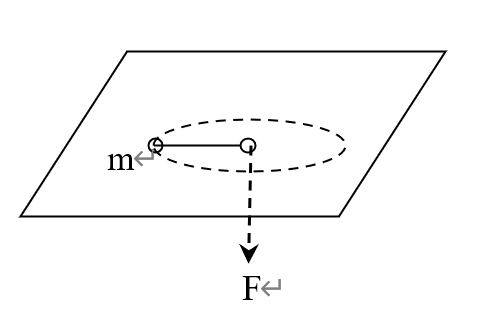
\includegraphics[width=0.15\textheight]{fig37}
            \caption{如图}\label{fig:37}
    \end{figure}
\end{enumerate}
\subsection*{二、选择题}
\begin{enumerate}
    \item 两个匀质圆盘$A$和$B$的半径分别为$R_A$和$R_B$, 若$R_A>R_B$, 但两圆盘的质量相同, 如两盘对通过盘心垂直于盘面轴的转动惯量各为$J_A$和$J_B$, 则有(\hspace{1pc})
    \fourch{$J_A>J_B$;}{$J_B>J_A$;}{$J_A=J_B$;}{不能确定.}
    \item 一长为$l$, 质量为$m$的直杆, 可绕通过其一端的水平光滑轴在竖直平面内作定轴转动, 在杆的另一端固定着一质量为$m$的小球, 如图所示\ref{fig:38}. 
    现将杆由水平位置无初转速地释放. 则杆刚被释放时的角加速度$\beta_0$为(\hspace{1pc})
    \fourch{$\frac{9g}{8l}$;}{$\frac{g}{l}$;}{$\frac{3g}{2l}$;}{$\frac{18g}{13l}$.}
    \begin{figure}[H]
        \centering
        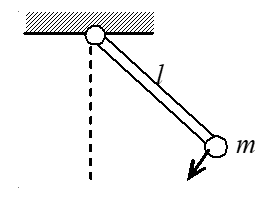
\includegraphics[width=0.10\textheight]{fig38}
            \caption{如图}\label{fig:38}
    \end{figure}
    \item 如图 \ref{fig:39}, 竖立的圆筒形转笼, 半径为$R$, 绕中心轴$OO^{'}$转动, 物块$A$紧靠在圆筒的内壁上, 物块与圆筒间的摩擦系数为$\mu$, 要使物块$A$不下落, 
    圆筒转动的角速度$\omega$至少应为(\hspace{1pc})
    \fourch{$\sqrt{\frac{\mu g}{R}}$;}{$\sqrt{\mu g}$;}{$\sqrt{\frac{g}{\mu R}}$;}{$\sqrt{\frac{g}{R}}$.}
    \begin{figure}[H]
        \centering
        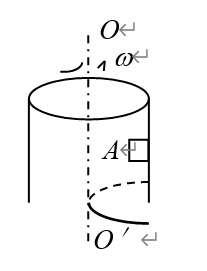
\includegraphics[width=0.15\textheight]{fig39}
            \caption{如图}\label{fig:39}
    \end{figure}
    \item 一飞轮以角速度$\omega_0$绕光滑固定轴旋转, 飞轮对轴的转动惯量为$J_1$, 另一静止飞轮突然和上述转动的飞轮啮合, 绕同一转轴转动, 该飞轮对轴的转动惯量为$2J_1$. 
    啮合后整个系统的动能为(\hspace{1pc})
    \fourch{$\frac{1}{3}J_1\omega_0^2$;}{$\frac{1}{6}J_1\omega_0^2$;}{$\frac{1}{2}J_1\omega_0^2$;}{$\frac{3}{2}J_1\omega_0^2$.}

\end{enumerate}
\subsection*{三、计算题}
\begin{enumerate}
    \item 如图所示 \ref{fig:40}, 一半径为$R$, 质量为$m$的均匀圆盘, 可绕水平固定光滑轴转动, 
    现以一轻绳绕在轮边缘, 绳的下端挂一质量为$m$的物体, 
    求圆盘从静止开始转动后, 它转过的角度和时间的关系.
    \begin{figure}[H]
        \centering
        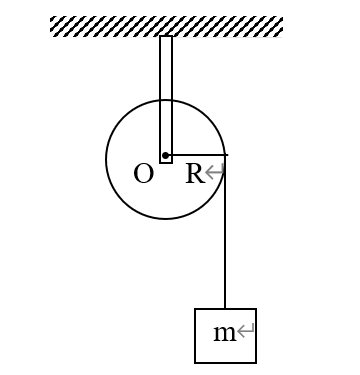
\includegraphics[width=0.15\textheight]{fig40}
            \caption{如图}\label{fig:40}
    \end{figure}
    \item 如图\ref{fig:41},质量为$M$, 长为$L$的均匀直杆可绕$O$轴在竖直平面内无摩擦地转动, 开始时杆处于自由下垂位置, 
    一质量为$m$的弹性小球水平飞来与杆下端发生完全弹性碰撞, 若$M>3m$, 且碰撞后, 杆上摆的最大角度为$\theta$, 则求:
    \begin{enumerate}
        \item[(1)] 小球的初速度$V_0$
        \item[(2)] 碰撞过程中杆给小球的冲量
    \end{enumerate}
        \begin{figure}[H]
            \centering
            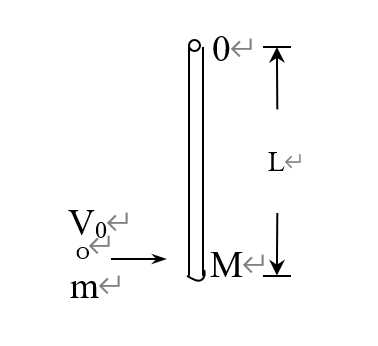
\includegraphics[width=0.15\textheight]{fig41}
                \caption{如图}\label{fig:41}
        \end{figure}
        
\end{enumerate}

\section{习题参考答案}
\subsection*{一、填空题}
\begin{enumerate}
    \item 如图 \ref{Fig:34}, 一长为$L$, 质量为$m$的匀质细杆, 两端分别固定质量为$m$和$2m$的小球,
    此系统在竖直平面内可绕过中点$O$且与杆垂直的水平光滑固定轴($O$轴)转动. 
    开始时杆与水平成$60^\circ$角, 处于静止状态 . 
    无初转速地释放以后, 杆球这一刚体系统绕$O$轴转动. 
    释放后, 当杆转到水平位置时, 刚体受到的合外力矩$M=\anl{$\frac{1}{2}mgL$}$.
    \begin{figure}[H]
        \centering
        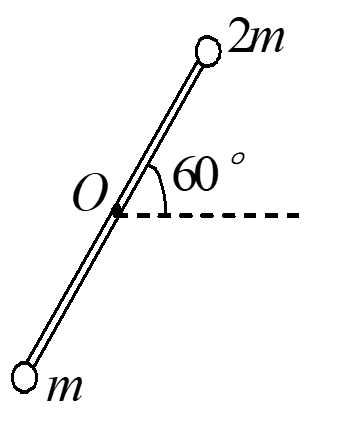
\includegraphics[width=0.15\textheight]{fig34}
            \caption{如图}\label{Fig:34}
    \end{figure}
    \begin{note}
        \textcolor{red}{$M=2mg\frac{L}{2}-mg\frac{L}{2}=\frac{1}{2}mgL$}
    \end{note}
    \item 如图 \ref{Fig:35}, 一定滑轮质量为$M$、半径为$R$, 对水平轴的转动惯量$J=(1/2)MR^2$.
    在滑轮的边缘绕一细绳, 绳的下端挂一物体. 
    绳的质量可以忽略且不能伸长, 滑轮与轴承间无摩擦, 
    物体下落的加速度为$a$.则绳中的张力$T=\anl{$\frac{1}{2}Ma$}$.
    \begin{figure}[H]
        \centering
        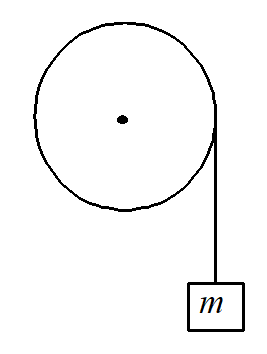
\includegraphics[width=0.15\textheight]{fig35}
            \caption{如图}\label{Fig:35}
    \end{figure}
    \begin{note}
        $TR=J\alpha$, $a=R\alpha$, $T=\frac{1}{2}Ma$
    \end{note}
    \item 一长为$L$质量为$m$的均质细杆, 两端附着质量分别为$m_1$和$m_2$
    的小球, 且$m_1>m_2$, 两小球直径$d_1$、$d_2$都远小于$L$, 
    此杆可绕通过中心并垂直于细杆的轴在竖直平面内转动, 
    则它对该轴的转动惯量为\underline{\makebox[11em]{$\frac{1}{12}(m+3m_1+3m_2)L^2$}}, 若将它由水平位置自静止释放, 
    则它在开始时刻的角加速度为多大\underline{\makebox[9em]{$\frac{6(m_1-m_2)g}{(m+3m_1+3m_2)L}$}}.
    \begin{note}
        \textcolor{red}{$\frac{1}{12}mL^2+m_1(\frac{L}{2})^2+m_2(\frac{L}{2})^2$, $M=\frac{L}{2}m_1g-\frac{L}{2}m_2g=J\alpha$}
    \end{note}
    \item 如图所示 \ref{Fig:36}, 一质量为$m$的质点自由落下的过程中某时刻具有速度$V$,
    此时它相对于$A$、$B$、$C$三个参考点的距离分别为$d_1、d_2、d_3$
    则质点对这三个参考点的角动量的大小, $L_A=\bnl{$mvd_1$}$, 
    $L_B=\bnl{$mvd_1$}$, $L_C=\bnl{$0$}$; 作用在质点上的重力对这三个点的力矩大小,
    $M_A=\bnl{$mgd_1$}$; $M_B=\bnl{$mgd_1$}$; $M_C=\bnl{$0$}$.
    \begin{figure}[H]
        \centering
        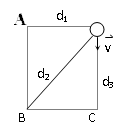
\includegraphics[width=0.15\textheight]{fig36}
            \caption{如图}\label{Fig:36}
    \end{figure}
    \item 哈雷慧星绕太阳的运动轨道为一椭圆, 太阳位于椭圆轨道的一个焦点上,它离太阳最近的距离是$r_1=8.75\times10^{10}m$, 此时的速率是$V_1=5.46\times10^4\cdots m\cdot S^{-1}$, 在离太阳最远的位置上的速率是
    $V_2=9.08\times 10^2 m·S^{-1}$, 此时它离太阳的距离是$r_2=\anl{$5.26\times 10^{12}$}$.
    \begin{note}
       \textcolor{red}{$mr_1v_1=mr_2v_2, r_2=\frac{v_1}{v_2}r_1=5.26\times 10^{12} m$}.
    \end{note}
    \item 假设卫星环绕地球中心作圆周运动, 则在运动过程中, 卫星对地球中心的角动量、动量、动能这三个量中守恒的是\anl{角动量、动能} .
    \item 如图 \ref{Fig:37}, 质量为$m$的小球, 拴于不可伸长的轻绳上, 在光滑水平桌面上作匀速圆周运动, 其半径为$R$, 角速度为$\omega$, 绳的另一端通过光滑的竖直管用手拉住, 如把绳向下拉$R/2$
    时角速度$\omega^{'}$为\anl{$\omega^{'}=4\omega$} , 在此过程中, 手对绳所作的功为\anl{$A=\frac{3}{2}mR^2\omega^2$} .
    \begin{figure}[H]
        \centering
        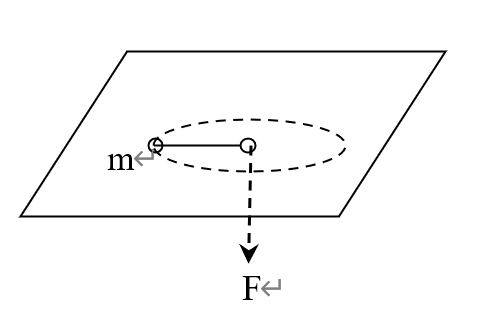
\includegraphics[width=0.15\textheight]{fig37}
            \caption{如图}\label{Fig:37}
    \end{figure}
    \begin{note}
        \textcolor{red}{$mR^2\omega=m(R/2)^2\omega^{'}, A=\frac{1}{2}m{v^{'}}^2-\frac{1}{2}mv^2=\frac{1}{2}m(\frac{R}{2}\cdot \omega^{'})^2-\frac{1}{2}m(R\omega)^2=\frac{3}{2}mR^2\omega^2$}.
    \end{note}
\end{enumerate}
\subsection*{二、选择题}
\begin{enumerate}
    \item 两个匀质圆盘$A$和$B$的半径分别为$R_A$和$R_B$, 若$R_A>R_B$, 但两圆盘的质量相同, 如两盘对通过盘心垂直于盘面轴的转动惯量各为$J_A$和$J_B$, 则有( A )
    \fourch{$J_A>J_B$;}{$J_B>J_A$;}{$J_A=J_B$;}{不能确定.}
    \begin{note}
        \textcolor{red}{均质圆盘\ \ $J=\frac{1}{2}mR^2$\qquad $\therefore J_A>J_B$}
    \end{note}
    \item 一长为$l$, 质量为$m$的直杆, 可绕通过其一端的水平光滑轴在竖直平面内作定轴转动, 在杆的另一端固定着一质量为$m$的小球, 如图所示\ref{Fig:38}. 
    现将杆由水平位置无初转速地释放. 则杆刚被释放时的角加速度$\beta_0$为( A )
    \fourch{$\frac{9g}{8l}$;}{$\frac{g}{l}$;}{$\frac{3g}{2l}$;}{$\frac{18g}{13l}$.}
    \begin{figure}[H]
        \centering
        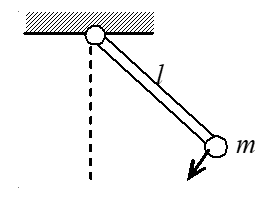
\includegraphics[width=0.10\textheight]{fig38}
            \caption{如图}\label{Fig:38}
    \end{figure}
    \begin{note}
        \textcolor{red}{$M=mgl+mg\frac{l}{2}=J\beta_0$, $J=\frac{1}{3}ml^2+ml^2$, $\beta_0=\frac{9g}{8l}$}
    \end{note}
    \item 如图 \ref{Fig:39}, 竖立的圆筒形转笼, 半径为$R$, 绕中心轴$OO^{'}$转动, 物块$A$紧靠在圆筒的内壁上, 物块与圆筒间的摩擦系数为$\mu$, 要使物块$A$不下落, 
    圆筒转动的角速度$\omega$至少应为( C )
    \fourch{$\sqrt{\frac{\mu g}{R}}$;}{$\sqrt{\mu g}$;}{$\sqrt{\frac{g}{\mu R}}$;}{$\sqrt{\frac{g}{R}}$.}
    \begin{figure}[H]
        \centering
        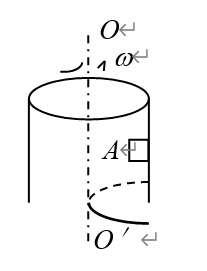
\includegraphics[width=0.15\textheight]{fig39}
            \caption{如图}\label{Fig:39}
    \end{figure}
    \begin{note}
        \textcolor{red}{$\because F=mR\omega^2$, $\therefore f \le \mu F=\mu mR\omega^2$, 恰好不掉下时有: $f=mg$, 故$\omega \ge \omega_{min}=\sqrt{\frac{g}{\mu R}}$}
    \end{note}
    \item 一飞轮以角速度$\omega_0$绕光滑固定轴旋转, 飞轮对轴的转动惯量为$J_1$, 另一静止飞轮突然和上述转动的飞轮啮合, 绕同一转轴转动, 该飞轮对轴的转动惯量为$2J_1$. 
    啮合后整个系统的动能为( B )
    \fourch{$\frac{1}{3}J_1\omega_0^2$;}{$\frac{1}{6}J_1\omega_0^2$;}{$\frac{1}{2}J_1\omega_0^2$;}{$\frac{3}{2}J_1\omega_0^2$.}
    \begin{note}
        \textcolor{red}{角动量守恒 $J_1w_0=(J_1+2J_1)\omega$\ \ $\omega=\frac{1}{3}\omega_0$, 动能\ $E_k=\frac{1}{2}(3J_1)\omega^2=\frac{1}{6}J_1\omega_0^2$}
    \end{note}
\end{enumerate}
\subsection*{三、计算题}
\begin{enumerate}
    \item 如图所示 \ref{Fig:40}, 一半径为$R$, 质量为$m$的均匀圆盘, 可绕水平固定光滑轴转动, 
    现以一轻绳绕在轮边缘, 绳的下端挂一质量为$m$的物体, 
    求圆盘从静止开始转动后, 它转过的角度和时间的关系.
    \begin{figure}[H]
        \centering
        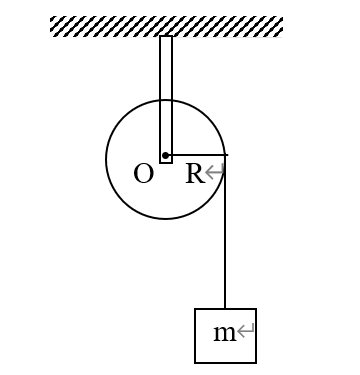
\includegraphics[width=0.15\textheight]{fig40}
            \caption{如图}\label{Fig:40}
    \end{figure}
    \begin{solution}
        看图: 
        \begin{figure}[H]
            \centering
            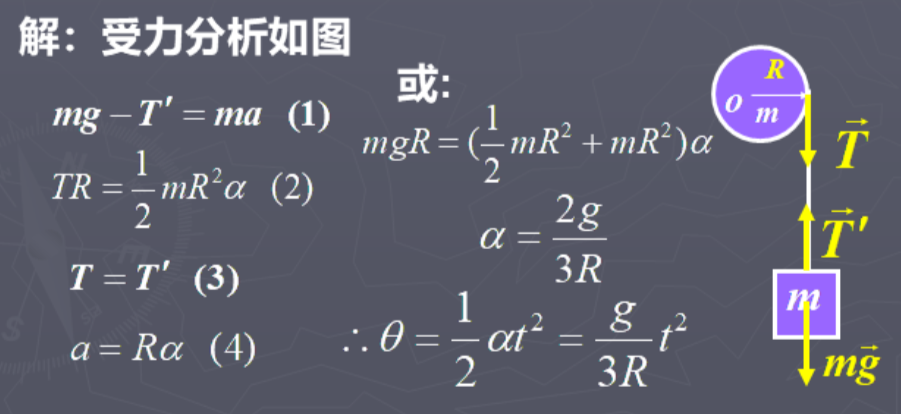
\includegraphics[width=0.48\textheight]{ans23}
        \end{figure}
    \end{solution}
    \item 如图\ref{Fig:41},质量为$M$, 长为$L$的均匀直杆可绕$O$轴在竖直平面内无摩擦地转动, 开始时杆处于自由下垂位置, 
    一质量为$m$的弹性小球水平飞来与杆下端发生完全弹性碰撞, 若$M>3m$, 且碰撞后, 杆上摆的最大角度为$\theta$, 则求:
    \begin{enumerate}
        \item[(1)] 小球的初速度$V_0$
        \item[(2)] 碰撞过程中杆给小球的冲量
    \end{enumerate}
        \begin{figure}[H]
            \centering
            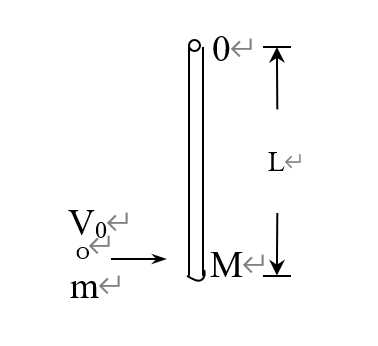
\includegraphics[width=0.15\textheight]{fig41}
                \caption{如图}\label{Fig:41}
        \end{figure}
        \begin{solution}
            看图: 
            \begin{figure}[H]
                \centering
                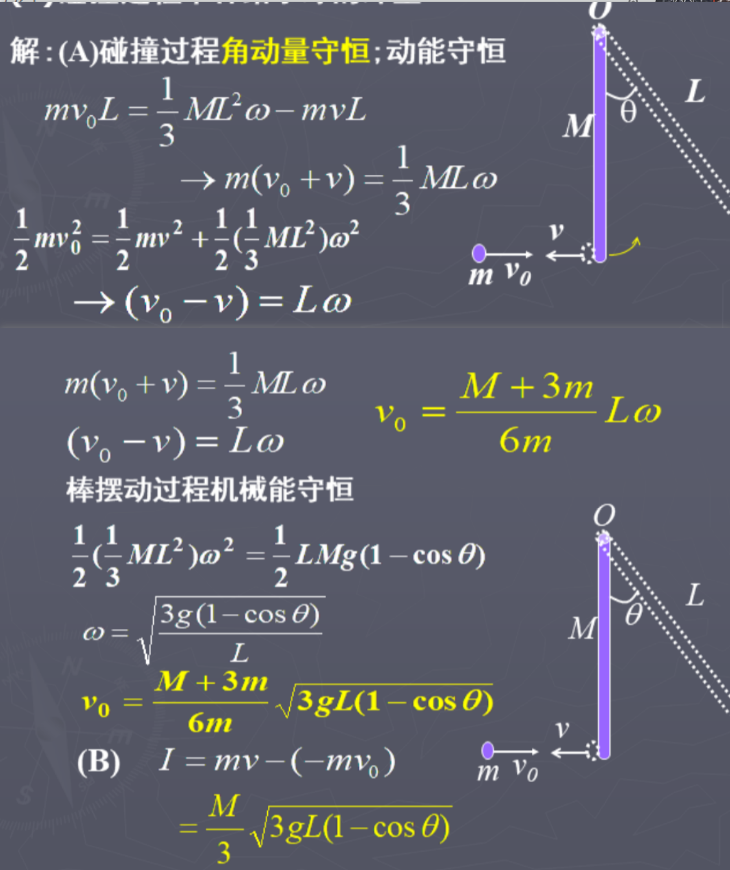
\includegraphics[width=0.48\textheight]{ans24}
            \end{figure}
        \end{solution}  
\end{enumerate}